%% \chapter[htoc-titlei][hhead-titlei]{htitlei}
%% -----------------------------------------------------------------------------
\chapter[Monte Carlo simulation][Monte Carlo simulation]{Monte Carlo simulation}
\label{ch:mc}

Monte Carlo (MC) simulations are an important tool for particle physics
experiments.
MC techniques are used to simulate physics processes that occur during
particle collisions.
These simulated events also include the interactions of the decay products
in the detector, and can be used to tune the selection of an analysis,
estimate the expected event yields and kinematic shapes, and ultimately,
evaluate the expected sensitivity of a particular search.
MC simulation of background and signal processes are used on \ATLAS.
This chapter introduces some of the basic concepts of event generation, but
focuses on the generation of the $B-L$ stop pairs from the model described in
Section~\ref{sec:theory_bl_extension}.

MC simulation of particle physics events can be broken into two major parts.
The first step is the event generation, described in
Section~\ref{sec:event_gen}.
In the event generation stage, the actual Physics processes that occur as a
result of the collision are simulated.
This includes the hard interaction as well as the resulting decay of any
unstable particles, and finally the hadronization of any decay products with
color charge.
As in the real detector, once the proton collisions are simulated, the decay
products travel through the detector, and may leave a measurable signature
which can be measured.
This involved material interactions with the detector, and is discussed in
Section~\ref{sec:det_sim}.

%% -----------------------------------------------------------------------------
\FloatBarrier
\section{Event Generation}
\label{sec:event_gen}

Before discussing the details of event generation, it is useful to first
introduce the concept of an ``event.''
At the LHC, beams of protons are accelerated in opposite directions, and
allowed to cross at specific locations as described in Section~\ref{sec:lhc}.
At each of these crossings, protons from the two beams collide with one
another, resulting in a spray of particles in the detector.
Each of these crossings represents a single event.
Figure~\ref{fig:mc_event} shows a pictorial representation of a simulated
$t\bar{t}H$ event, and Figure~\ref{fig:data_event} shows a $t\bar{t}H$
candidate event as reconstructed in the \ATLAS\ detector.

\begin{figure}[p]
  \centering
  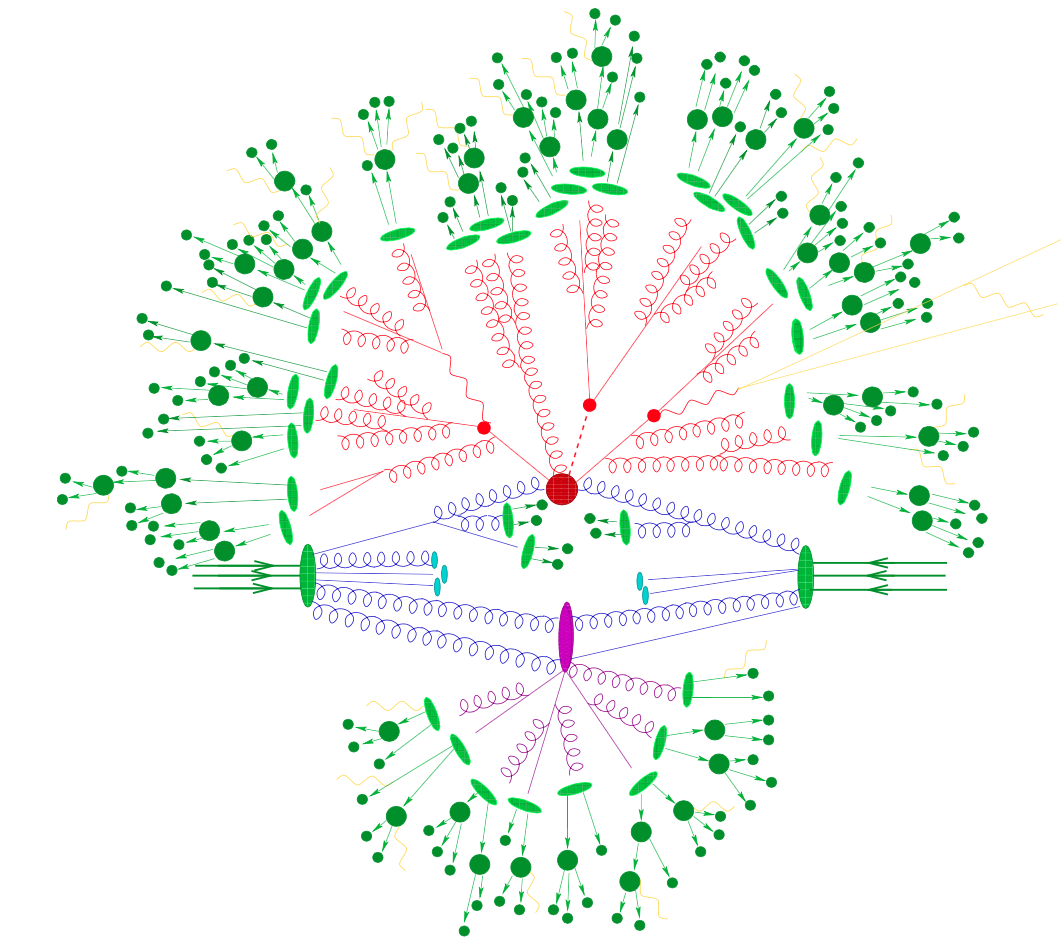
\includegraphics[width=\textwidth, clip=true, trim=0 0 0 0]
  {figs/mc_gen/full_mc_event.png}
  \caption[
    Pictorial representation of a $t\bar{t}H$ event as produced by an event
    generator~\cite{Gleisberg:2008ta}.
  ]{
    Pictorial representation of a $t\bar{t}H$ event as produced by an event
    generator.
    The hard interaction (big red blob) is followed by the decay of both top
    quarks and the Higgs boson (small red blobs).
    Additional hard QCD radiation is produced (red) and a secondary
    interaction takes place (purple blob) before the final-state partons
    hadronize (light green blobs) and hadrons decay (dark green blobs).
    Photon radiation occurs at any stage (yellow)~\cite{Gleisberg:2008ta}.
  }
  \label{fig:mc_event}
\end{figure}

\begin{figure}[ht]
  \centering
  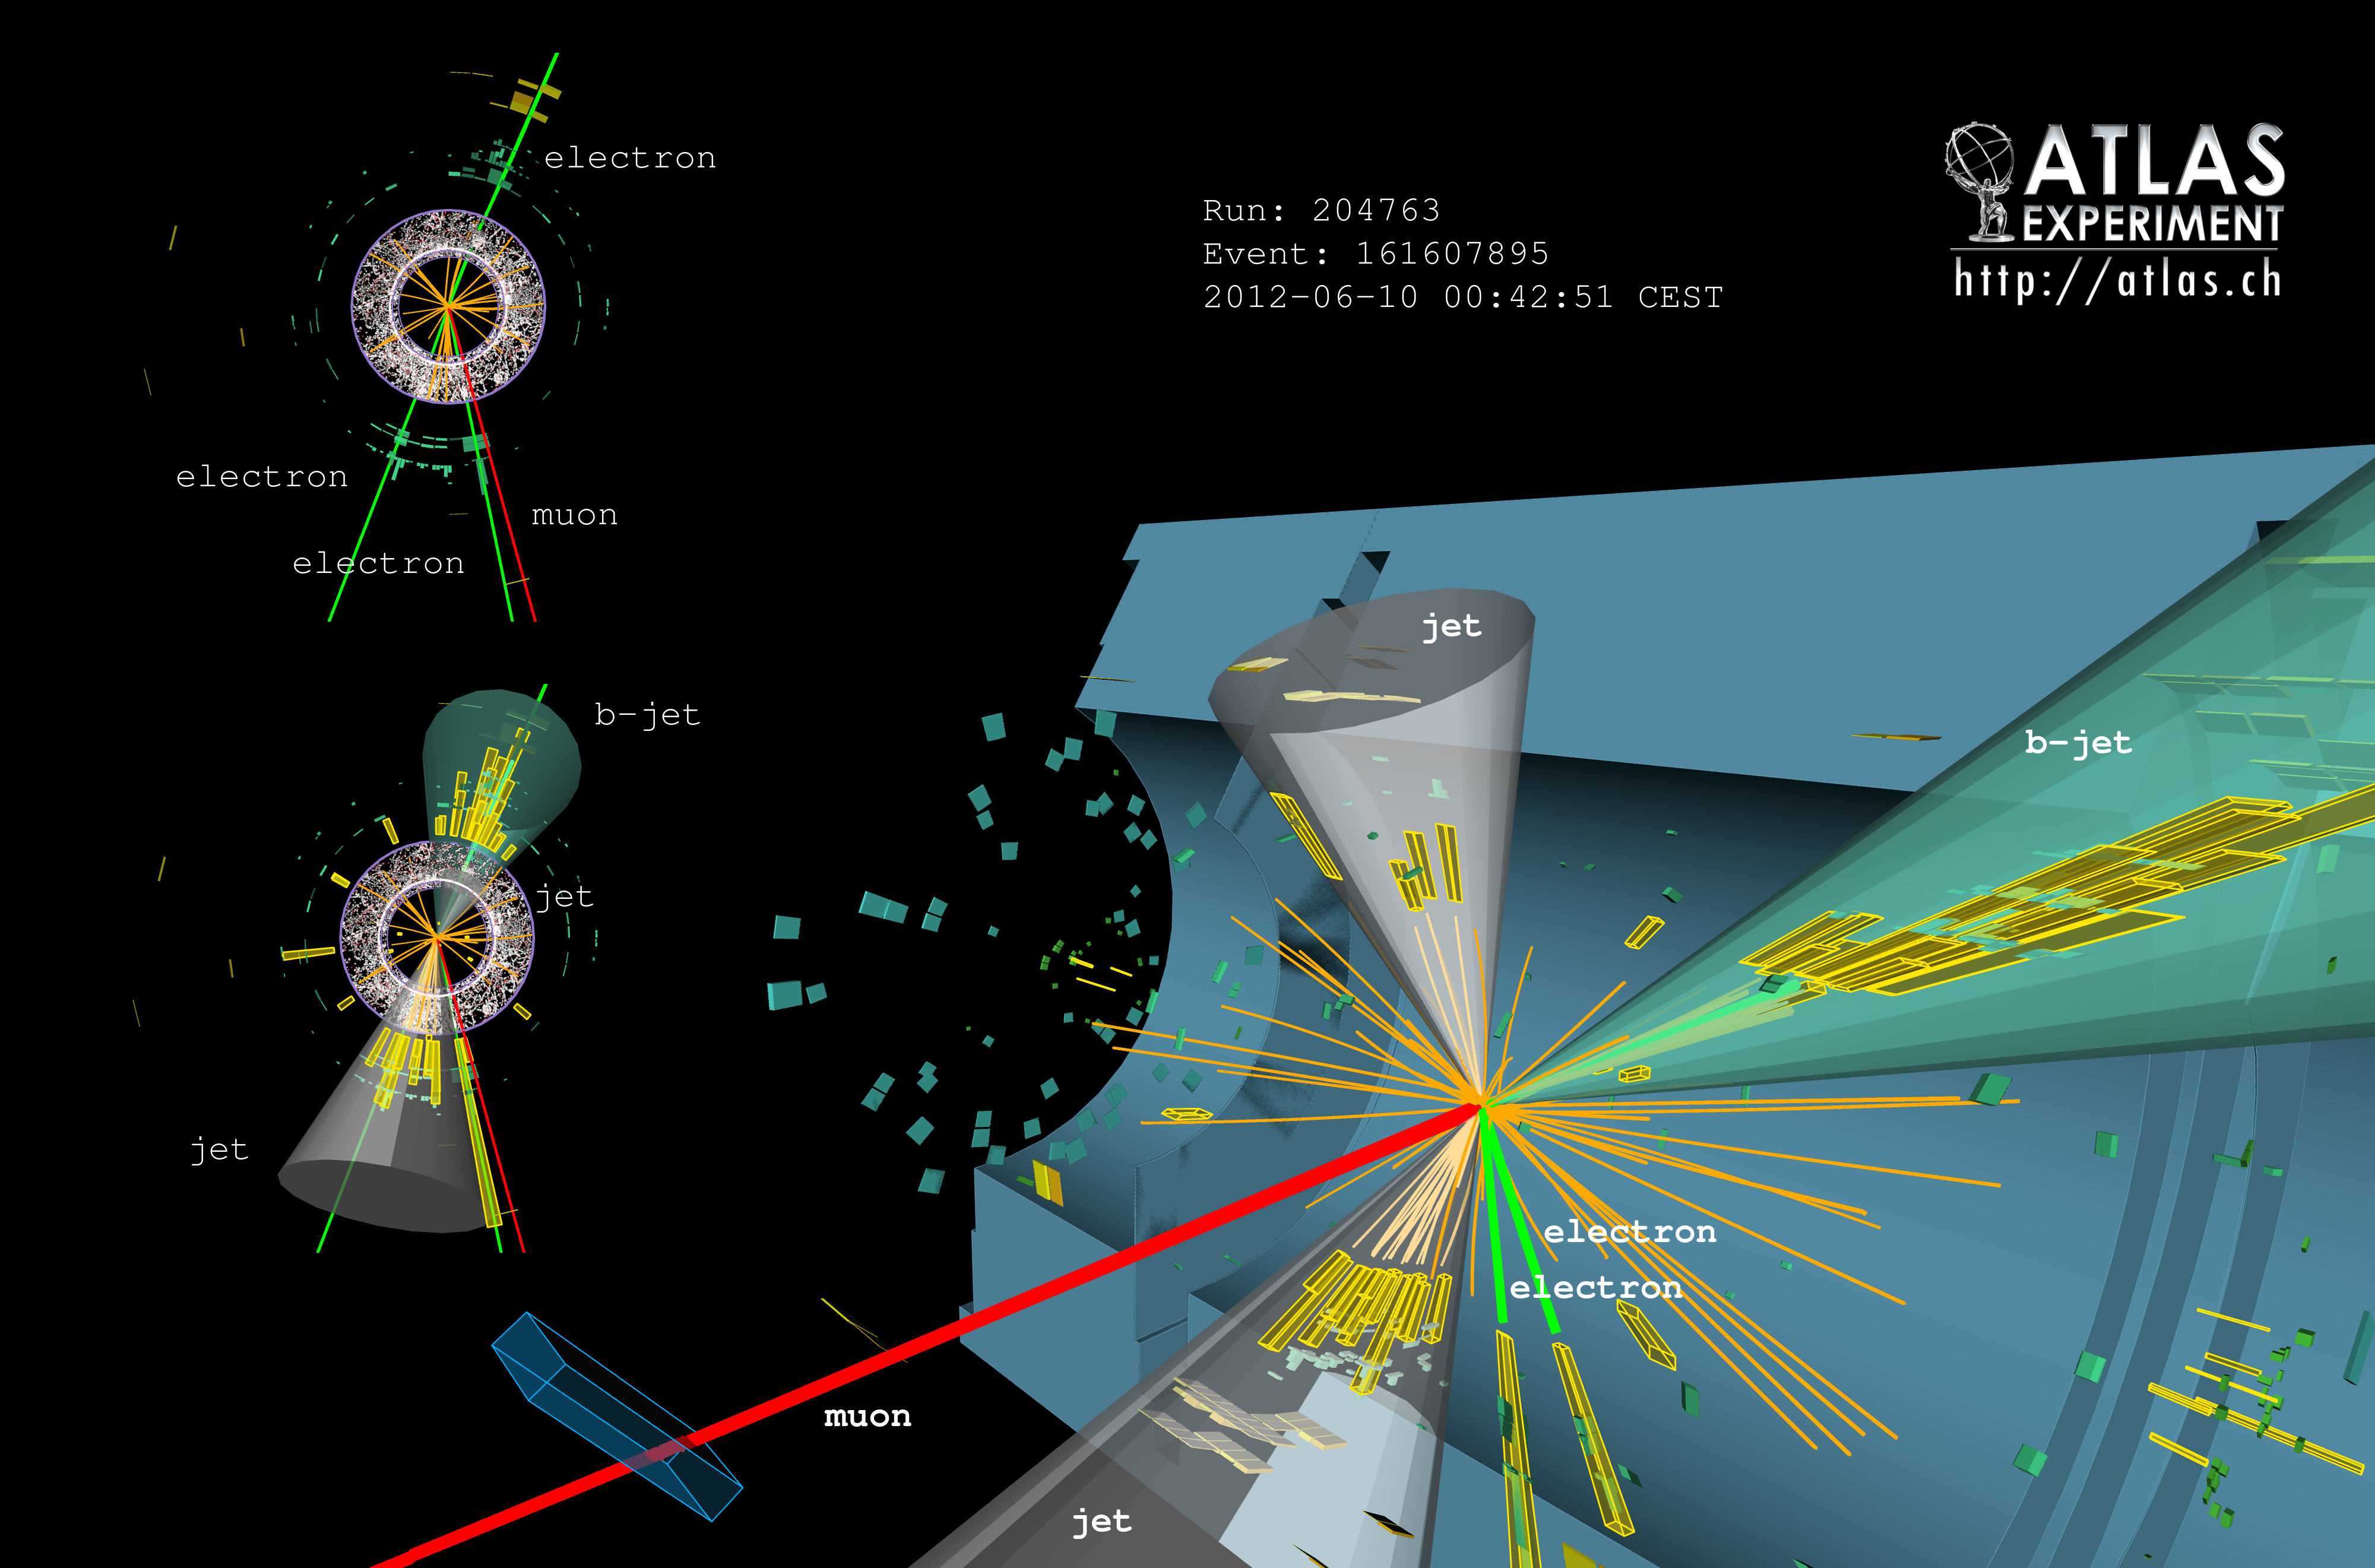
\includegraphics[width=\textwidth, clip=true, trim=0 0 0 0]
  {figs/mc_gen/tth_event.png}
  \caption{
    Candidate $t\bar{t}H$ event, observed in the
    \ATLAS\ detector~\cite{Aad:2015iha}.
  }
  \label{fig:data_event}
\end{figure}

Looking more closely at the interactions taking place, one notices that,
rather than the full protons interacting with each other, the interactions
take place between the constituent quarks and gluons within the two protons.
In some cases, there is a ``hard interaction,'' or an inelastic scattering
where additional particles are created.
This is mathematically represented by the ``matrix element'' calculation.
As the protons pass through each other, there are also soft interactions
between the constituent partons in a process called the ``underlying event.''
The underlying event produces charged particles and jets in the detector, in
addition to those coming from the hard interaction.

%% - - - - - - - - - - - - - - - - - - - - - - - - - - - - - - - - - - - - - - -
\FloatBarrier
\subsection{Parton distribution function}
\label{sec:pdf}

It is often said a proton is made up of three quarks and the gluons holding
them together.
Due to the QCD effects, this is actually a simplification, and additional
quarks and gluons are produced within hadrons, and have a large impact 
on the interactions between colliding hadrons.
The parton content with hadrons is described by a parton distribution
function (PDF).

The PDF of a proton, $p(x, \mu^2)$, gives the probability that, at a particular
energy scale $\mu^2$, a particular parton, $p$, is found inside the proton, with
a fraction of the total momentum between $x$ and $x+dx$.
A proton must satisfy the following sum rules in order to have the correct
``valance quark'' content.
\begin{align}
  \int_0^1 \left( u(x, \mu^2) - \bar{u}(x, \mu^2) \right) dx & = 2, \\
  \int_0^1 \left( d(x, \mu^2) - \bar{d}(x, \mu^2) \right) dx & = 1, \\
  \int_0^1 \left( q(x, \mu^2) - \bar{q}(x, \mu^2) \right) dx & = 0,
\end{align}
Where $q$ is any other quark flavor.

PDFs are tuned to the observed data at collider experiments such as \ATLAS,
and improve over time as more data is collected at higher energy scales.
Two example PDFs, provided by the NNPDF group, are shown in
Figure~\ref{fig:pdfs}, corresponding to different energy scales.
The CTEQ 6L1 PDF tune is used for the simulated stop pair production in the
analysis described in this thesis.

\begin{figure}
  \centering
  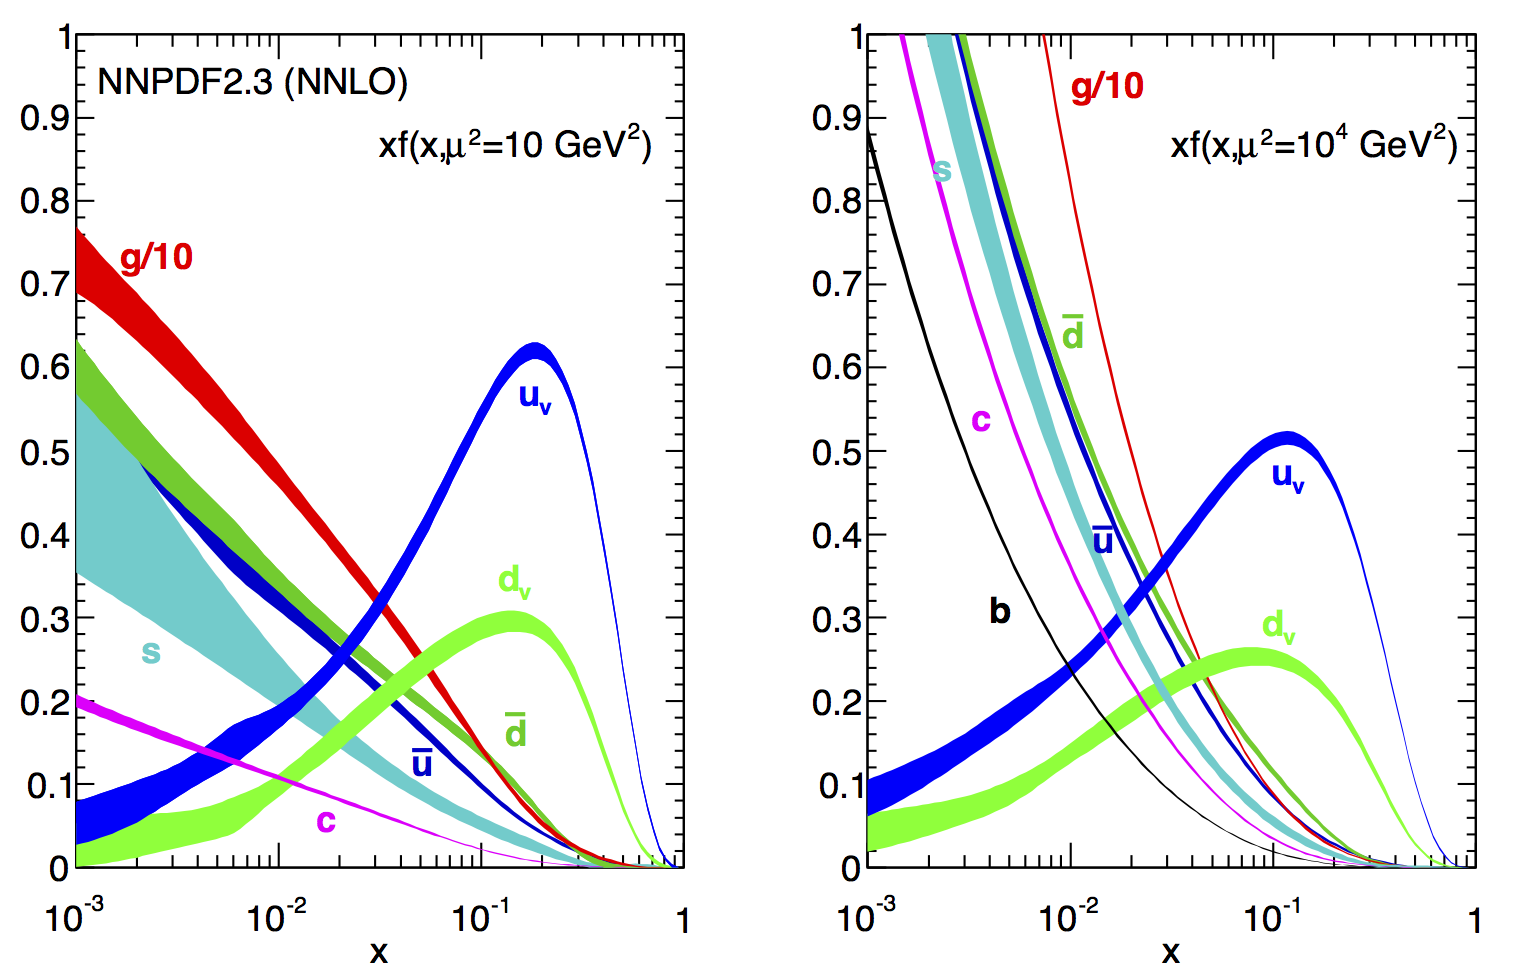
\includegraphics[width=0.80\textwidth]{figs/mc_gen/pdfs.png}
  \caption{Parton distribution function (PDF) distributions for different
    parton species within the proton as obtained by the NNPDF collaboration.
    The two PDF distributions are obtained for different energy
    scales ($\mu^2$)~\cite{nnpdf}.
  }
  \label{fig:pdfs}
\end{figure}


%% - - - - - - - - - - - - - - - - - - - - - - - - - - - - - - - - - - - - - - -
\FloatBarrier
\subsection{Underlying event}
\label{sec:underlying_event}

The underlying event makes up the parts of the collision event resulting from
the breakup of the initial-state protons after partons are knocked out during
the hard interaction.
A schematic of a di-jet
the underlying event highlighted in a di-jet event is shown in
Figure~\ref{fig:underlying_event}.
The different lines represent the incoming protons (blue), the hard
interaction (red), the underlying event (black), and initial and final state
radiation (pink).
The hard interaction includes the incoming partons which interaction, and
the resulting outgoing particles which go on to form the final-state jets.

\begin{figure}
  \centering
  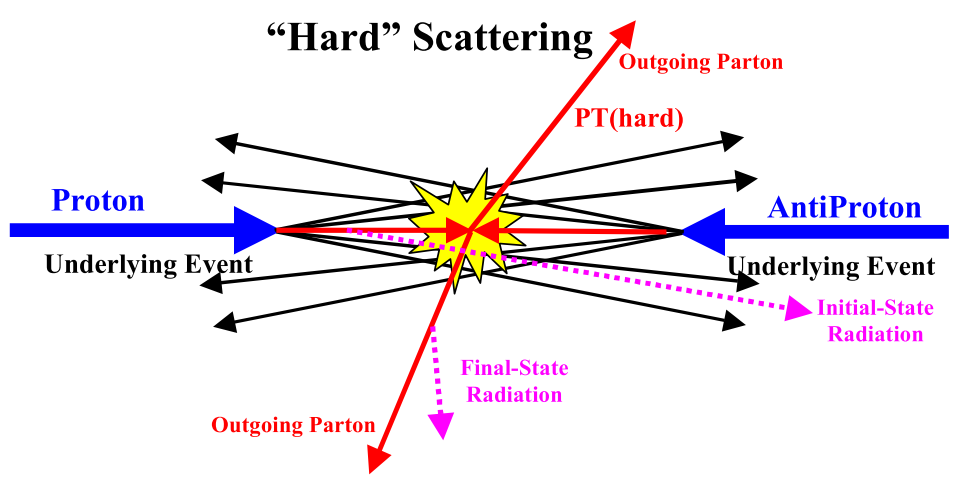
\includegraphics[width=0.80\textwidth]{figs/mc_gen/underlying_event.png}
  \caption{
    Schematic of a di-jet event with the underlying event in a
    proton-anti-proton collision~\cite{Field:2002vt}.
  }
  \label{fig:underlying_event}
\end{figure}

Once the proton is broken apart during the collision, the ``beam remnants''
will be scattered, and potentially undergo additional, softer interactions.
This is known as ``multiple parton interactions,'' and leads to additional
activity in the detector, including additional charged particles and jets.
There can also be initial or final state radiation associated with the
beam remnant, which is also classified as part of the underlying
event~\cite{Field:2002vt}.

Modeling the underlying event requires adequate tunes of the proton PDFs
and the soft interaction terms, and is beyond the scope of this thesis.

%% - - - - - - - - - - - - - - - - - - - - - - - - - - - - - - - - - - - - - - -
\FloatBarrier
\subsection{Hard interaction}
\label{sec:matrix_element}

The ``hard interaction'' refers to the process within a collision event
with the highest $\sum \pt$ when summing over all the outgoing particles
from a particular interaction.
This is usually the most interesting part of the event, and when generating
MC simulation of simulation events, the events are generally categorized by
the hard interaction process.

The cross section of a generic scattering process $a\,b \to F+X$ is given by
\begin{equation}
  \sigma_{a\,b \to F+X} \propto
  \left|\mathcal{M}_{a\,b \to F+X}\right|^2 \Phi_{F},
\end{equation}
where $a$ and $b$ are the incoming partons, $F$ is the final state, and $X$
represents anything else that may be in the event, such as additional quarks or
gluons which go on to form jets.
The production cross section is given in terms of a matrix
element, $\mathcal{M}_{a\,b \to F+X}$, and a phase space term, $\Phi_F$.
The matrix element term is $\mathcal{M}_{a\,b \to F+X}$ is the scattering
amplitude, and is given by the Fourier Transform of the scattering potential.
The phase space is related to the density of final states.

Several software tools exist to calculate scattering cross section by
generating the relevant diagrams, calculating the these matrix element terms,
and integrating over the phase space for the final states.
The tools then use these cross sections and Monte Carlo techniques to simulate
collision events, which have the same production cross section and kinematics
as events one expects to observe in real collision data.
The simulated events mimic the realistic collision events in that they have
incoming and outgoing particles, and any unstable particles are allowed to
decay.
Each of the particles in the simulated event are represented by four-vectors,
with values for the mass and momentum.
Examples of these software tools include \sherpa, \powheg, and \madgraph.
In particular, \madgraph\ is used to generate the simulated signal events for
the analysis described in this thesis.

%% - - - - - - - - - - - - - - - - - - - - - - - - - - - - - - - - - - - - - - -
\FloatBarrier
\subsection{Parton shower}
\label{sec:parton_shower}

The matrix element calculations are a useful tool in calculating the cross
sections for infrared safe processes such as $Z$~boson or di-jet production,
but there can be cases, such as collinear radiation, where the calculations
diverge.
These divergences are clearly non-physical, as such infinities don't exist in
nature, so a different approach is needed in this regime.
A common technique is the ``parton shower'' method implemented by software
tools such as \pythia.
The basic idea of the parton shower method can be illustrated in the context of
gluon radiation off of a quark.
Similar to Bremsstrahlung radiation of QED, a quark will radiate gluons as it
travels.
\pythia\ models the quark as moving along its trajectory, and in each step,
there is some probability of radiating a gluon with a given momentum.
Each time a gluon is radiated, the quark will lose momentum, until a
threshold is reached, and the quark will begin to hadronize rather than
continue to radiate.

%% - - - - - - - - - - - - - - - - - - - - - - - - - - - - - - - - - - - - - - -
\FloatBarrier
\subsection{Jet matching}
\label{sec:jet_matching}

As with the matrix element calculation, the parton shower method is not without
its problems.
The parton shower is not as well suited for calculating the cross section
for very hard processes, where the momentum transfer is large, but this is
exactly the regime where the matrix element calculations is accurate.
For this reason, both methods are used when simulating collision events for
use in analyses.
The matrix element is used to generate the hard process and the initial decay
products, then the parton shower takes over to add any additional radiation
below the cutoff scale of the matrix element calculation.

Naively combining the matrix element calculation the parton shower technique
introduces a potential double counting of diagrams as illustrated in
Figure~\ref{fig:mc_double_counting}.
Figure~\ref{fig:mc_double_counting} shows three diagrams for the production
of a $Z$~boson, associated with additional partons, which lead to jets in the
final state.
In all cases, the matrix element technique is used to generate the $Z$~boson
production along with one or two additional partons.
Parton showering is applied to the additional partons, but not the initial
state particles to simplify the example.

In the left scenario only a single additional parton in the matrix element
calculation, and the parton shower method is used to determine the soft
collinear radiation off of the quark.
One would like to add scenarios like the middle diagram, which includes a
second additional parton in the matrix element calculation.
The middle diagram includes a hard emission of a gluon in the matrix element
calculation, and parton showering is used to include the soft radiation from
the gluon.
If these are the only two diagrams, there would be no problem, however, the
parton shower will occasionally result in a hard, large-angle gluon emission
from the quark, as shown in the right scenario.
This leads to the possibility of double counting since both the middle and
right diagrams generate the same process~\cite{Salam:2010zt}.

\begin{figure}
  \centering
  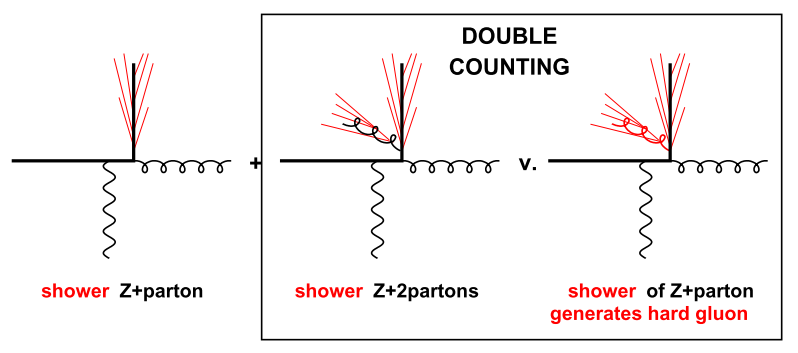
\includegraphics[width=0.8\textwidth]{figs/mc_gen/double_conting.png}
  \caption[
    Illustration of the double counting issue that arises when combining the
    matrix element and parton shower event generation
    techniques~\cite{Salam:2010zt}.
  ]{
    Illustration of the double counting issue that arises when combining the
    matrix element and parton shower event generation techniques.
    The diagrams show $Z$~boson production associated with one or two
    additional partons included in the matrix element
    calculation~\cite{Salam:2010zt}.
  }
  \label{fig:mc_double_counting}
\end{figure}

As mentioned before, the matrix element technique is well suited for processes
with large momentum transfer, while parton showering is better for soft,
collinear emissions.
It is necessary to define a cutoff for when an additional parton emission is
``hard enough'' to be included in the matrix element calculation.
This procedure of eliminating double counting is called ``jet matching,'' and
many methods exist.
While the implementation differs for each of the algorithms, the basic approach
for each of the methods is illustrated in Figure~\ref{fig:mc_jet_matching}.
A scale is defined for each of the additional partons produced, either in the
matrix element calculation, or through the parton showering.
The definition of the scale is different for each algorithm, but is it related
to the momentum of the parton and the angle at which it is radiated.
For simplicity, the scale will be referred to as $k_\mathrm{T}$.

Two thresholds are defined, called $Q_\mathrm{ME}$ and $Q_\mathrm{merge}$,
where $Q_\mathrm{ME} \leq Q_\mathrm{merge}$.
These thresholds are mark the cutoff between the matrix element and parton
showering stages of the event generation process.
Partons generated in the matrix element calculation are required to have
$k_\mathrm{T} \geq Q_\mathrm{ME}$.
Similarly, the parton shower step may only add additional partons with
$k_\mathrm{T} \leq Q_\mathrm{ME}$~\cite{Salam:2010zt}.

The Shower $k_\mathrm{T}$ is used when generating stop pair
events~\cite{Alwall:2008qv}.
The thresholds are chosen such that
$Q_\mathrm{ME} = Q_\mathrm{merge} = \frac{m_{\tilde{t}}}{4}$.

\begin{figure}
  \centering
  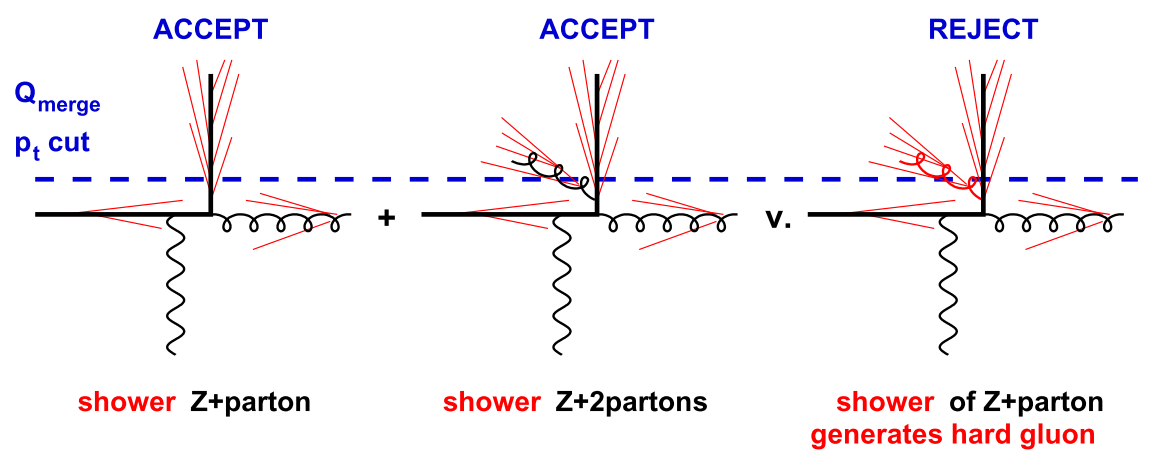
\includegraphics[width=0.8\textwidth]{figs/mc_gen/jet_matching.png}
  \caption[
    Illustration of the jet matching technique used to eliminate the double
    counting issue shown in
    Figure~\ref{fig:mc_double_counting}~\cite{Salam:2010zt}.
  ]{
    Illustration of the jet matching technique used to eliminate the double
    counting issue shown in
    Figure~\ref{fig:mc_double_counting}.
    The $Q_\mathrm{merge}$ cutoff scale is shown as a dashed blue line, and
    events failing this requirement are rejected~\cite{Salam:2010zt}.
  }
  \label{fig:mc_jet_matching}
\end{figure}


% {\color{red} Talk about matching. Probably use several figures to help explain
%   this topic. Probably also talk about these DJR plots, and how we want them
%   to look}
% 
% {\color{red} Add info about HFOR here}

%% -----------------------------------------------------------------------------
\FloatBarrier
\section{Detector simulation}
\label{sec:det_sim}

Event generation is only the first step in producing MC simulation samples.
The interactions of the particles as they pass through the detector must also
be simulated.
The interactions of the particles with the material in the detector are
simulated in one of two ways, know as full simulation or fast simulation.

In the full simulation, a model of the \ATLAS\ detector is built within \geant4.
The simulation includes not only the active parts of the detector used in
measuring particles, but also the support structure and services such as cables
and electronics.
The particles are propagated through the simulated detector, and allowed to
interact in a way similar to a real particle traveling through the
\atlas\ detector.
Simulated interaction in any of the subsystems result in simulated
measurements, which can be inputted into the reconstruction software, just as
data from the real detector.

Much like the full simulation, the fast simulation uses \geant4 to simulate the
interactions of particles through the inner detector and the muon systems.
The two models differ in the treatment of the calorimeter.
Rather than fully simulate the showers in the calorimeter, the fast simulation
uses parameterized shower shapes for particles that interact with the
electromagnetic and hadronic calorimeters.

A more complete discussion of the \atlas\ simulation setup can be found
in Reference~\cite{ATLASSimulation}.

